\chapter{Introdução}

\section{Motivação}

O avanço da tecnologia e o aumento de sua complexidade trouxe a necessidade de um enorme tráfego de dados entre dispositivos. Com isso surgiram alguns problemas, como o congestionamento de dados, interferências no transporte e aumento do número de cabos para comunicação, entre outros, que levam a uma diminuição na velocidade de transmissão de dados. Isso, além de uma maior demora no recebimento, dificulta tarefas do nosso dia a dia que estão ficando cada vez mais prioritárias, é o caso de transmissões em tempo real de vídeos 4K, utilizado muito em vídeo conferências, \textit{streaming} e também na medicina, área na qual é preciso ter o máximo de detalhes na imagem e baixa latência.

Isso gera a necessidade do desenvolvimento de sistemas de transmissão mais avançados e em bandas de frequência que permitam essa alta taxa de transmissão, o que pode ser obtido através de ondas milimétricas. As ondas milimétricas são ondas que encontram-se na faixa de frequência entre 24-100GHz, portanto possuem uma grande banda a ser explorada mas com alguns desafios na transmissão e recepção devido a altas frequências. 

Foi com essa necessidade que o professor Gustavo Rehder nos propôs o desafio de desenvolver uma comunicação sem fio em 60 GHz, um projeto que é continuação de outro projeto de formatura de 2017, feito por \citeauthor{TCC} e orientado também pelo Professor Gustavo Rehder. Os autores fizeram a seleção dos componentes utilizados, estruturaram a arquitetura da solução, conseguiram desenvolver a interface de configuração entre o computador e o transceptor comercial. Entretanto, devido a problemas de fabricação do transmissor e receptor, não foi possível realizar os testes de transmissão e a modulação do vídeo a ser enviado ao transmissor.

O principal problema foram curto-circuitos nos pinos do circuito integrado utilizado, isso aconteceu devido a precisão necessária para soldar o componente, que possui encapsulamento do tipo \textit{ball grid array (BGA)}, e a falta de um método preciso para realizar a metalização das vias de ligação entre os dois lados condutores da placa de circuito impresso. 

\section{Objetivos}

Este projeto terá como objetivo a pesquisa, o desenvolvimento e a fabricação de um transmissor e um receptor de ondas milimétricas, mais especificamente na faixa de 60 GHz, para a transmissão em tempo real de vídeos em alta qualidade sem compressão. Nessa frequência, conseguimos uma baixa latência devido a alta taxa de transmissão mas também uma qualidade do sinal devido a faixa de 60 GHz que é absorvida pelo oxigênio e que resulta em menos interferências no sinal, o que não é possível em baixas frequências.

Para a fabricação do projeto  serão estudadas maneiras de realizar a deposição de cobre nas paredes internas das vias, revisão do projeto e fabricação das placas transmissora e receptora, estudo modulação de vídeos para envio e testes de transmissão sem fio na faixa de 60 GHz entre os dois dispositivos. Todos os processos de fabricação e testes serão feito com apoio da equipe e infraestrutura do Laboratório de Microeletrônica da USP (LME).

\section{Árvore de Objetivos}

Uma árvore objetivos é a representação gráfica do objetivo geral do projeto mostrando os objetivos específicos, que são os meios para chegar no objetivo principal. Para atingir esse objetivo, realizando a comunicação de um vídeo em 4k foi elaborada a seguinte árvore de objetivos:

\begin{figure}[htbp]
    \centering
    %\captionsetup{justification=centering}
    \caption{Árvore de objetivos do projeto}
    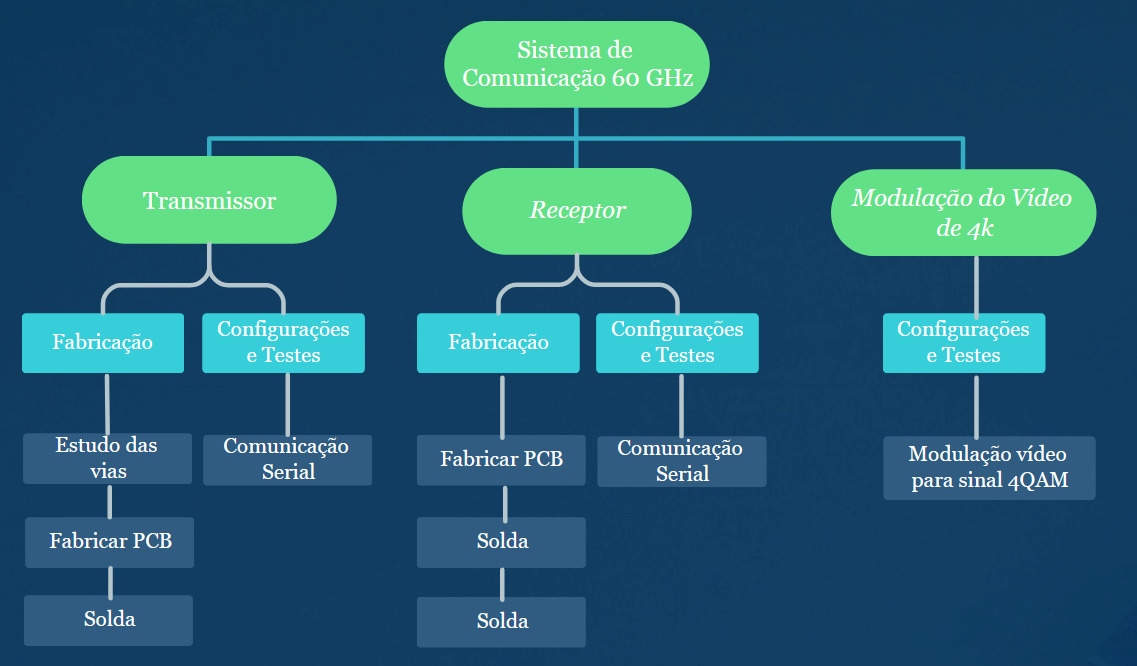
\includegraphics[width = \linewidth - 1cm]{arvoredeobjetivos.jpeg}
    
    \source{De autoria própria}
    \centering
    \label{Árvore}
\end{figure}